\documentclass[11pt, a4paper]{article}

\usepackage[english]{babel}
\usepackage{sleek}
\usepackage{common}

\title{Introduction to Artificial Intelligence (INFO8006)}
\subtitle{Exercises 4 -- Reasoning over time}
\date{\today}

\begin{document}

\maketitle

\section*{Learning outcomes}

At the end of this session you should be able to
\begin{itemize}[noitemsep]
    \item formulate a Markov model for discrete-time reasoning problems;
    \item define the simplifying assumptions of Markov processes;
    \item define and apply prediction, filtering and smoothing in Markov processes;
    \item apply the simplified matrix algorithm(s) to hidden Markov models;
    \item define the Kalman filter assumptions and manipulate multivariate Gaussian distributions.
\end{itemize}

\section{Umbrella World (AIMA, Section 15.1.1)}

You are a security guard stationed at a secret underground installation. You want to know whether it is raining today, but your only access to the outside world occurs each morning when you see the director coming in with, or without, an umbrella. For each day $t$, the evidence is a single variable $Umbrella_t \in \cbk{1, 0}$, \ie{} whether the umbrella appears or not, and the (hidden) state is a single variable $Rain_t \in \cbk{1, 0}$, \ie{} whether it is raining or not.

You believe that from one day $t - 1$ to the next $t$, the chances that the weather stays the same are \SI{70}{\percent}. You also believe that the director brings his umbrella \SI{90}{\percent} of the time when it is raining, and \SI{20}{\percent} of the time otherwise.

\begin{enumerate}
    \item You would like to represent your umbrella world as a Markov model. What formal assumptions correspond to your beliefs ?

    \begin{solution}
        The first belief describes the umbrella world as a \emph{first-order Markov process}, such that
        \begin{equation*}
            P(R_t \knowing R_{1:t-1}) = P(R_t \knowing R_{t-1}),
        \end{equation*}
        \ie{} $R_t$ is independent from $R_{1:t - 2}$ given $R_{t-1}$. The second belief is equivalent to a \emph{first-order sensor Markov assumption}, implying that
        \begin{equation*}
            P(U_t \knowing R_{1:t}, U_{1:t-1}) = P(U_t \knowing R_{t}).
        \end{equation*}
    \end{solution}

    \item Sketch a Bayesian network structure describing the umbrella world and provide the transition and sensor models.

    \begin{solution}
        \begin{figure}[H]
            \centering
            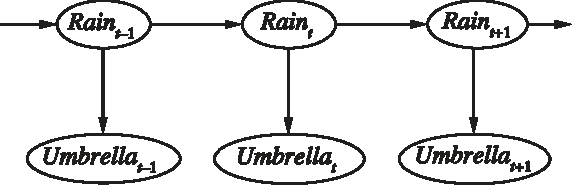
\includegraphics[width=0.6\textwidth]{figures/e4_umbrella.pdf}
        \end{figure}

        \begin{table}[H]
            \begin{subtable}[c]{0.495\textwidth}
                \centering
                \begin{tabular}{c|c}
                    \toprule
                     $R_{t-1}$ & $P(R_t = 1 \knowing R_{t-1})$ \\
                     \midrule
                     1 & 0.7 \\
                     0 & 0.3 \\
                    \bottomrule
                \end{tabular}
            \end{subtable}
            \begin{subtable}[c]{0.495\textwidth}
                \centering
                \begin{tabular}{c|c}
                    \toprule
                     $R_t$ & $P(U_t = 1 \knowing R_t)$ \\
                     \midrule
                     1 & 0.9 \\
                     0 & 0.2 \\
                    \bottomrule
                \end{tabular}
            \end{subtable}
        \end{table}
    \end{solution}

    \item Express the distributions $P(R_{t + 1} \knowing R_{t-1})$, $P(U_t \knowing R_{t-1})$ and $P(R_t \knowing R_{t-1}, U_t)$ in terms of the transition and sensor models.

    \begin{solution}
        \begin{align*}
            P(R_{t + 1} \knowing R_{t-1}) & = \sum_{r_t} P(R_{t + 1} \knowing r_t) P(r_t \knowing R_{t-1}) \\
            & = \mat{0.7 & 0.3 \\ 0.3 & 0.7} \mat{0.7 & 0.3 \\ 0.3 & 0.7} = \mat{0.58 & 0.42 \\ 0.42 & 0.58} \\
            P(U_t \knowing R_{t-1}) & = \sum_{r_t} P(U_t \knowing R_{t-1}, r_t) P(r_t \knowing R_{t-1}) \\
            & = \sum_{r_t} P(U_t \knowing r_t) P(r_t \knowing R_{t-1}) \\
            & = \mat{0.9 & 0.2 \\ 0.1 & 0.8} \mat{0.7 & 0.3 \\ 0.3 & 0.7} = \mat{0.69 & 0.41 \\ 0.31 & 0.59} \\
            P(R_t \knowing R_{t-1}, U_t) & = \frac{P(U_t \knowing R_{t-1}, R_t) P(R_t \knowing R_{t-1})}{P(U_t \knowing R_{t-1})} \\
            & = \frac{P(U_t \knowing R_t) P(R_t \knowing R_{t-1})}{P(U_t \knowing R_{t-1})}
        \end{align*}
    \end{solution}

    \item Suppose you observe an unending sequence of days on which the umbrella appears. Show that, as the days go by, the probability of rain on the current day tends monotonically towards a fixed point. Calculate this fixed point.

    \begin{solution}
        We are asked to prove that $x_t = P(R_t = 1 \knowing U_{1:t} = 1)$ tends monotonically (with respect to $t$) towards a fixed point $x^*$. To do so, we need to find the value of $x_t$, which corresponds to apply \emph{filtering} on the Markov model defined by the umbrella world. On this basis, we have
        \begin{alignat*}{2}
            && P(R_t \knowing U_{1:t} = 1) & = \alpha P(U_t = 1 \knowing R_t) \sum_{r_{t-1}} P(R_t \knowing r_{t-1}) P(r_{t-1} \knowing U_{1:t-1}  = 1) \\
            &&& = \alpha \mat{0.9 & 0 \\ 0 & 0.2} \mat{0.7 & 0.3 \\ 0.3 & 0.7} P(R_{t-1} \knowing U_{1:t-1} = 1) \\
            \Leftrightarrow \quad && \mat{x_{t} \\ 1 - x_{t}} & = \alpha \mat{0.63 & 0.27 \\ 0.06 & 0.14} \mat{x_{t-1} \\ 1 - x_{t-1}} \\
            &&& = \alpha \mat{0.27 + (0.63 - 0.27) \, x_{t-1} \\ 0.14 + (0.06 - 0.14) \, x_{t-1}} \\
            &&& = \frac{1}{0.41 + 0.28 \, x_{t-1}} \mat{0.27 + 0.36 \, x_{t-1} \\ 0.14 - 0.08 \, x_{t-1}} .
        \end{alignat*}
        Then, if there is a fixed point $x^* \in [0, 1]$, it satisfies
        \begin{alignat*}{2}
            && x^* & = \frac{0.27 + 0.36 \, x^*}{0.41 + 0.28 \, x^*} \\
            \Leftrightarrow \quad && 0.41 \, x^* + 0.28 \, {x^*}^2 & = 0.27 + 0.36 \, x^* \\
            \Leftrightarrow \quad && 0 & = 0.28 \, {x^*}^2 + 0.05 \, x^* - 0.27 \\
            \Rightarrow \quad && x^* & = \frac{-0.05 + \sqrt{0.05^2 + 4 \times 0.27 \times 0.28}}{2 \times 0.28} \approx \num{0.897} .
        \end{alignat*}
        To show that $x_t$ tends monotonically towards $x^*$, it is sufficient to prove that $x_t$ is always between $x^*$ and $x_{t-1}$, \ie{}
        \begin{equation*}
            (x^* - x_t) (x_t - x_{t-1}) > 0,
        \end{equation*}
        when $x_{t-1} \neq x^*$, which is left as an exercise to the motivated reader.
    \end{solution}

    \item Now consider forecasting further and further into the future, given $t$ umbrella observations. Is there a fixed point ? If yes, compute its exact value.

    \begin{solution}
        We are asked to forecast the rain probability $x_k = P(R_{t + k} = 1 \knowing U_{1:t} = 1)$, \ie{} to perform \emph{prediction}. We have
        \begin{alignat*}{2}
            && P(R_{t+k} \knowing U_{1:t} = 1) & = \sum_{r_{t+k-1}} P(R_{t+k} \knowing r_{t+k-1}) P(r_{t+k-1} \knowing U_{1:t} = 1) \\
            &&& = \mat{0.7 & 0.3 \\ 0.3 & 0.7} P(R_{t+k-1} \knowing U_{1:t} = 1) \\
            \Leftrightarrow \quad && \mat{x_k \\ 1 - x_k} & = \mat{0.7 & 0.3 \\ 0.3 & 0.7} \mat{x_{k - 1} \\ 1 - x_{k - 1}} .
        \end{alignat*}
        By symmetry, we find the fixed point $x^* = 0.5$, which highlights the fact that, without new evidences, uncertainty about the states accumulates.
    \end{solution}
\end{enumerate}

\newpage

\section{The coins}

You are in a room containing 3 precious biased gold coins $a$, $b$ and $c$. You inspect the coins and notice that the coins $a$, $b$ and $c$ have a head probability of \qty{80}{\percent}, \qty{50}{\percent} and \qty{20}{\percent}, respectively.

Another person enters the room, takes the coins and put them into a bag. They draw a coin from the bag and tell you that they will repeat 4 times the same routine: hide their hand in the bag and either keep the current coin with probability $\frac{2}{3}$ or replace it by another, then toss it and show you the result. They proceed and the sequence of results are heads, heads, tail, heads. If you answer right to the following questions they will give you the coins.

\begin{enumerate}
    \item Provide a hidden Markov model (HMM) that describes the process.

    \begin{solution}
        \begin{itemize}
            \item The hidden state at time $t$ is $X_t \in \cbk{a, b, c}$ and represents the tossed coin.

            \item The evidence at time $t$ is $E_t \in \cbk{0, 1}$ and represents the result (heads or tail) of the toss. We have $e_1 = e_2 = e_4 = 0$ and $e_3 = 1$.

            \item The prior vector
                \begin{equation*}
                    f_0 = P(X_0) = \mat{\frac{1}{3} & \frac{1}{3} & \frac{1}{3}}^T
                \end{equation*}

            \item The transition matrix
                \begin{equation*}
                    T = P(X_t \knowing X_{t-1}) = \mat{
                        \frac{2}{3} & \frac{1}{6} & \frac{1}{6} \\
                        \frac{1}{6} & \frac{2}{3} & \frac{1}{6} \\
                        \frac{1}{6} & \frac{1}{6} & \frac{2}{3}
                    }
                \end{equation*}

            \item The sensor matrix
                \begin{equation*}
                    B = P(E_t \knowing X_t) = \mat{
                        0.8 & 0.5 & 0.2 \\
                        0.2 & 0.5 & 0.8
                    }
                \end{equation*}
        \end{itemize}
    \end{solution}

    \item What are the probabilities of the last coin given the sequence of evidences?

    \begin{solution}
        We are asked to calculate the distribution $f_t = P(X_t \knowing e_{1:t})$ for $t = 4$. Applying Bayes filter, we have
        \begin{alignat*}{2}
            && P(X_t \knowing e_{1:t}) & = \alpha P(e_t \knowing X_t, e_{1:t-1}) P(X_t \knowing e_{1:t-1}) \\
            &&& = \alpha P(e_t \knowing X_t, e_{1:t-1}) \sum_{x_{t-1}} P(X_t \knowing x_{t-1}, e_{1:t-1}) P(x_{t-1} \knowing e_{1:t-1}) \\
            &&& = \alpha P(e_t \knowing X_t) \sum_{x_{t-1}} P(X_t \knowing x_{t-1}) P(x_{t-1} \knowing e_{1:t-1}) \\
            \Leftrightarrow \quad && f_t & = \alpha \, O_t \, T \, f_{t-1}
        \end{alignat*}
        where $O_t = \diag(P(e_t | X_t))$ is the observation matrix. By substitution,
        \begin{equation*}
                O_1 = O_2 = O_4 = \mat{0.8 & 0 & 0 \\ 0 & 0.5 & 0 \\ 0 & 0 & 0.2} \quad \text{and} \quad O_3 = \mat{0.2 & 0 & 0 \\ 0 & 0.5 & 0 \\ 0 & 0 & 0.8} .
        \end{equation*}
        Then, to calculate $f_4$, we first need $f_1$, $f_2$ and $f_3$.
        \begin{align*}
            f_1 & = \alpha_1 \, O_1 \, T \, f_0 = \alpha_1 \mat{0.8 & 0 & 0 \\ 0 & 0.5 & 0 \\ 0 & 0 & 0.2} \mat{
                \frac{2}{3} & \frac{1}{6} & \frac{1}{6} \\
                \frac{1}{6} & \frac{2}{3} & \frac{1}{6} \\
                \frac{1}{6} & \frac{1}{6} & \frac{2}{3}
            } \mat{\frac{1}{3} \\ \frac{1}{3} \\ \frac{1}{3}} = \alpha_1 \mat{\frac{4}{15} \\ \frac{1}{6} \\ \frac{1}{15}} = \mat{\frac{8}{15} \\ \frac{1}{3} \\ \frac{2}{15}} \\
            f_2 & = \alpha_2 \, O_2 \, T \, f_1 = \dots \\
            f_3 & = \alpha_3 \, O_3 \, T \, f_2 = \dots \\
            f_4 & = \alpha_4 \, O_4 \, T \, f_3 = \dots \approx \mat{0.472 & 0.374 & 0.154}^T
        \end{align*}
    \end{solution}

    \item What are the probabilities of the first coin given the sequence of evidences? And of the first coin tossed?

    \begin{solution}
        We are asked to calculate the distribution $P(X_k \knowing e_{1:t})$ for $t = 4$ and $k = 0$. As $k < t$ this corresponds to \emph{smoothing} our belief of the past. We have
        \begin{align*}
            P(X_k \knowing e_{1:t}) & = \alpha P(X_k, e_{k + 1:t} \knowing e_{1:k}) \\
            & = \alpha P(e_{k + 1:t} \knowing X_k, e_{1:k}) P(X_k \knowing e_{1:k}) \\
            & = \alpha P(e_{k + 1:t} \knowing X_k) P(X_k \knowing e_{1:k})
        \end{align*}
        As we already know $f_k = P(X_k \knowing e_{1:k})$, we only need to compute $b_k = P(e_{k + 1:t} \knowing X_k)$. We have
        \begin{alignat*}{2}
            && P(e_{k + 1:t} \knowing X_k) & = \sum_{x_{k + 1}} P(x_{k + 1} \knowing X_k) P(e_{k + 1:t} \knowing X_k, x_{k + 1}) \\
            &&& = \sum_{x_{k + 1}} P(x_{k + 1} \knowing X_k) P(e_{k + 1} \knowing x_{k + 1}) P(e_{k + 2:t} \knowing x_{k + 1}) \\
            \Leftrightarrow \quad && b_k & = T^T \, O_{k + 1} \, b_{k + 1}
        \end{alignat*}
        where $b_t = b_4 = P(anything \knowing X_4) = \mat{1 & 1 & 1}^T$. Therefore, to calculate $b_0$, we first need $b_3$, $b_2$ and $b_1$.
        \begin{align*}
            b_3 & = T^T \, O_{4} \, b_4 = \mat{
                \frac{2}{3} & \frac{1}{6} & \frac{1}{6} \\
                \frac{1}{6} & \frac{2}{3} & \frac{1}{6} \\
                \frac{1}{6} & \frac{1}{6} & \frac{2}{3}
            } \mat{0.8 & 0 & 0 \\ 0 & 0.5 & 0 \\ 0 & 0 & 0.2} \mat{1 \\ 1 \\ 1} = \mat{0.65 \\ 0.5 \\ 0.35} \\
            b_2 & = T^T \, O_{3} \, b_3 = \dots \\
            b_1 & = T^T \, O_{2} \, b_2 = \dots \\
            b_0 & = T^T \, O_{1} \, b_1 = \dots \approx \mat{0.076 & 0.055 & 0.035}^T
        \end{align*}
        Eventually,
        \begin{align*}
            P(X_0 \knowing e_{1:4}) & = \alpha b_0 \times f_0 \approx \mat{0.457 & 0.331 & 0.212}^T \\
            P(X_1 \knowing e_{1:4}) & = \alpha b_1 \times f_1 \approx \mat{0.580 & 0.329 & 0.091}^T
        \end{align*}
    \end{solution}

    \item What is the most likely sequence of tossed coins?

    \begin{solution}
        The most likely sequence $x_{1:t}^*$ given the sequence of evidences $e_{1:t}$ is the one that satisfies
        \begin{equation*}
            x_{1:t}^* = \arg \max_{x_{1:t}} P(x_{1:t} \knowing e_{1:t})
        \end{equation*}
        or, equivalently,
        \begin{align*}
            x_k^* & = \arg \max_{x_k} \sbk*{ \max_{x_{1:k-1}} P(x_{1:k}, x^*_{k+1:t} \knowing e_{1:t}) } \\
            & = \arg \max_{x_k} \sbk*{ \max_{x_{1:k-1}} \alpha P(x_{1:k}, x^*_{k+1:t}, e_{k+1:t} \knowing e_{1:k}) } \\
            & = \arg \max_{x_k} \sbk*{ \max_{x_{1:k-1}} \alpha P(e_{k+1:t} \knowing x_{1:k}, x^*_{k+1:t}, e_{1:k}) P(x^*_{k+1:t} \knowing x_{1:k}, e_{1:k}) P(x_{1:k} \knowing e_{1:k}) } \\
            & = \arg \max_{x_k} \sbk[\bigg]{ \max_{x_{1:k-1}} \underbrace{\alpha P(e_{k+1:t} \knowing x^*_{k+1:t}) P(x^*_{k+2:t} \knowing x^*_{k+1})}_{\text{constant}} P(x^*_{k+1} \knowing x_{k}) P(x_{1:k} \knowing e_{1:k}) } \\
            & = \arg \max_{x_k} P(x^*_{k+1} \knowing x_{k}) \sbk*{ \max_{x_{1:k-1}} P(x_{1:k} \knowing e_{1:k}) } \\
            & = \arg \max_{x_k} P(x^*_{k+1} \knowing x_{k}) \, m_k(x_k)
        \end{align*}
        where
        \begin{align*}
            m_k & = \max_{x_{1:k-1}} P(x_{1:k-1}, X_k \knowing e_{1:k}) \\
            & = \max_{x_{1:k-1}} \alpha P(x_{1:k-1}, X_k, e_k \knowing e_{1:k-1}) \\
            & = \max_{x_{1:k-1}} \alpha P(e_t \knowing x_{1:k-1}, X_t, e_{1:k-1}) P(X_k \knowing x_{1:k-1}, e_{1:k-1}) P(x_{1:k-1} \knowing e_{1:k-1}) \\
            & = \max_{x_{1:k-1}} \alpha P(e_k \knowing X_k) P(X_k \knowing x_{k-1}) P(x_{1:k-1} \knowing e_{1:k-1}) \\
            & = \alpha P(e_k \knowing X_k) \max_{x_{k-1}} P(X_k \knowing x_{k-1}) \max_{x_{1:k - 2}} P(x_{1:k-1} \knowing e_{1:k-1}) \\
            & = \alpha P(e_k \knowing X_k) \max_{x_{k-1}} P(X_k \knowing x_{k-1}) \, m_{k-1}(x_{k-1})
        \end{align*}
        and $m_1 = P(X_1 \knowing e_1) = f_1$. Therefore, we can iteratively build the vectors $m_1$, $m_2$, \dots, $m_t$ to find the most likely last state
        \begin{equation*}
            x_t^* = \arg \max_{x_t} m_t(x_t)
        \end{equation*}
        and, then, the most likely sequence with
        \begin{equation*}
            x_k^* = \arg \max_{x_k} P(x^*_{k + 1} \knowing x_k) \, m_k(x_k) .
        \end{equation*}
    \end{solution}

\end{enumerate}

\newpage

\section{September 2019 (AIMA, Ex 15.13 and 15.14)}

A professor wants to know if students are getting enough sleep. Each day, the professor observes whether the students sleep in class, and whether they have red eyes. The professor has the following hypotheses:
\begin{itemize}
    \item The prior probability of getting enough sleep, with no observations, is \num{0.7}.
    \item The probability of getting enough sleep on night $t$ is \num{0.8} given that the student got enough sleep the previous night, and \num{0.3} otherwise.
    \item The probability of having red eyes is \num{0.2} if the student got enough sleep, and \num{0.7} otherwise.
    \item The probability of sleeping in class is \num{0.1} if the student got enough sleep, and \num{0.3} otherwise.
\end{itemize}
The professor asks you to answer the following questions:

\begin{enumerate}
    \item Formulate the environment and hypotheses as a dynamic Bayesian network that the professor could use to detect sleep deprived students, from a sequence of observations. Provide the associated probability tables.

    \item Reformulate the dynamic Bayesian network as a hidden Markov model that has only a single observation variable. Give the complete probability tables for the model.

    \item For the sequence $e_{1:3}$ of observations \enquote{no red eyes, not sleeping in class}, \enquote{red eyes, not sleeping in class} and
    \enquote{red eyes, sleeping in class}, calculate the distributions $P(EnoughSleep_t \knowing e_{1:t})$ and $P(EnoughSleep_t \knowing e_{1:3})$ for $t \in \cbk{1, 2, 3}$.
\end{enumerate}

\newpage

\section{Super Spring Ultra Pro Max XXL}

The \enquote{Foire de Liège} has a new attraction called \enquote{Super Spring Ultra Pro Max XXL} which consists in a ball hanging from a spring. The participants take seat in the ball locked at some position. The ball is then released and pulled by the spring which makes it oscillate back and forth. After a few seconds, the ball is stopped by magnetic brakes. You notice that the final position of the ball is different each time. As the ball is opaque, you wonder if it is possible for the participants to guess where the ball stopped, given their perception of acceleration.

You more or less remember your Newtonian mechanics class and model the movement of the ball as a series of transitions
\begin{align*}
    p_t & = p_{t-1} + \Delta t \, \dot{p}_{t - 1} + \frac{1}{2} {\Delta t}^2 \, \ddot{p}_{t - 1} \\
    \dot{p}_t & = \dot{p}_{t - 1} + \Delta t \, \ddot{p}_{t - 1} \\
    \ddot{p}_t & = g - \kappa \, p_{t - 1} - \eta \, \dot{p}_{t - 1} + \tau
\end{align*}
where $p_t$, $\dot{p}_t$ and $\ddot{p}_t$ are respectively the position, velocity and acceleration of the ball at timestep $t$, $\Delta t$ is the time elapsed between $t-1$ and $t$, $g$ is earth's surface gravity, $\kappa$ is the stiffness of the spring, $\eta$ is the linear drag coefficient of the air and $\tau \sim \N(0, \sigma_\tau^2)$ is the random thrust caused by the wind. You estimate that the ball starts \qty{10 \pm 0.5}{\meter} below the top of the spring with a negligible speed \qty{0 \pm 0.1}{\meter\per\second} and an acceleration $g - \kappa 10 \pm \sigma_\tau$. You also assume that the human perception of acceleration follows an unbiased Gaussian distribution.

\begin{enumerate}
    \item You wish to predict the state of the ball given the perceptions of a participant. Define the components of a Kalman filter in this context.

    \begin{solution}
        The Kalman filter is a special case of the continuous Bayes filter, which assumes
        \begin{itemize}
            \item a Gaussian prior
            \begin{equation*}
                p(x_0) = \N(\mu_0, \Sigma_0),
            \end{equation*}
            \item a linear Gaussian transition model
            \begin{equation*}
                p(x_t \knowing x_{t - 1}) = \N(A x_{t - 1} + b, \Sigma_x)
            \end{equation*}
            \item and a linear Gaussian sensor model
            \begin{equation*}
                p(e_t \knowing x_t) = \N(C x_t + d, \Sigma_e).
            \end{equation*}
        \end{itemize}
        In a \href{https://en.wikipedia.org/wiki/Multivariate_normal_distribution}{multivariate Gaussian distribution} $x = \mat{x_1 & x_2 & \dots & x_n}^T \sim \N(\mu, \Sigma)$, the first argument is the \emph{mean vector} and the second is the \emph{covariance matrix}. The mean vector is simply the vector of the variables' mean, \ie{} $\mu_i = \E\sbk{x_i}$. An element $\Sigma_{ij}$ of the covariance matrix is the covariance between the variables $x_i$ and $x_j$, \ie{} $\Sigma_{ij} = \E\sbk{(x_i - \mu_i) (x_j - \mu_j)}$. Interestingly, $\Sigma_{ii} = \E\sbk{(x_i - \mu_i)^2} = \V\sbk{x_i}$, meaning that the diagonal elements of $\Sigma$ are the variables' variance. Importantly, if $x_i$ is independent from $x_j$, their covariance is null by definition, \ie{} $\Sigma_{ij} = 0$.

        In our case, the state $x_t$ is a 3-dimensional vector $\mat{p_t & \dot{p}_t & \ddot{p}_t}^T$ and according to the provided information, the prior is defined by
        \begin{equation*}
            \mu_0 = \mat{10 \\ 0 \\ g - \kappa 10} \quad \text{and} \quad \Sigma_0 = \mat{0.5^2 & 0 & 0 \\ 0 & 0.1^2 & 0 \\ 0 & 0 & \sigma_\tau^2} .
        \end{equation*}
        Then, our transition model is defined by
        \begin{equation*}
            A = \mat{1 & \Delta t & \frac{1}{2} {\Delta t}^2 \\ 0 & 1 & \Delta t \\ -\kappa & - \eta & 0}, \quad b = \mat{0 \\ 0 \\ g} \quad \text{and} \quad \Sigma_x = \mat{0 & 0 & 0 \\ 0 & 0 & 0 \\ 0 & 0 & \sigma_\tau^2} .
        \end{equation*}
        It should be noted that only the acceleration has a non-null variance in $\Sigma_x$, since the transitions of the position and speed are considered \emph{deterministic}.

        Concerning the sensor model, the evidence is a perturbed, but unbiased, perception of the acceleration, that is
        \begin{align*}
            e_t & \sim \N(\ddot{p}_t, \sigma_e^2) ,
        \end{align*}
        which translates to
        \begin{equation*}
            C = \mat{0 & 0 & 1}, \quad d = 0 \quad \text{and} \quad \Sigma_e = \sigma_e^2 .
        \end{equation*}
    \end{solution}

    \item Express the distribution $p(x_t \knowing e_{1:t})$ with respect to the components defined previously.

    \begin{solution}
        This task corresponds exactly to filtering, \ie{} inferring the distribution
        \begin{align*}
            p(x_t \knowing e_{1:t}) & = \alpha \, p(e_t \knowing x_t, e_{1:t-1}) \, p(x_t \knowing e_{1:t-1}) \\
            & = \alpha \, p(e_t \knowing x_t) \int p(x_t \knowing x_{t-1}) \, p(x_{t-1} \knowing e_{1:t-1}) \d{x_{t-1}} .
        \end{align*}
        We notice that the latter expression depends on the sensor model $p(e_t \knowing x_t)$, the transition model $p(x_t \knowing x_{t-1})$ and our previous belief $p(x_{t-1} \knowing e_{1:t-1})$. When $t = 1$, this belief is the prior $p(x_0)$ and is a (multivariate) Gaussian distribution. But, from the cheat sheet for Gaussian models (slide 51, lecture 6), we know that if we have a Gaussian distribution $p(x) = \N(\mu_x, \Sigma_x)$ and a linear Gaussian condition distribution $p(y \knowing x) = \N(A x + b, \Sigma_y)$, the marginal $p(y)$ and the posterior $p(x \knowing y)$ are also Gaussian and take the form
        \begin{align*}
            p(y) & = \int p(y \knowing x) \, p(x) \d{x} = \N\rbk*{A \mu_x + b, \Sigma_y + A \Sigma_x A^T} \\
            p(x \knowing y) & = \alpha \, p(y \knowing x) \, p(x) = \N\rbk*{\Sigma \rbk*{A^T \Sigma_y^{-1} (y - b) + \Sigma_x^{-1} \mu_x}, \Sigma}
        \end{align*}
        with $\Sigma = \rbk*{\Sigma_x^{-1} + A^T \Sigma_y^{-1} A}^{-1}$. Then, by induction, all beliefs $p(x_t | e_{1:t})$ are Gaussian and we have
        \begin{align*}
            p(x_t | e_{1:t-1}) & = \int p(x_t \knowing x_{t-1}) \, p(x_{t-1} \knowing e_{1:t-1}) \d{x_{t-1}} = \N\rbk[\Big]{\underbrace{A \mu_{t-1} + b}_{\mu_*}, \underbrace{\Sigma_x + A \Sigma_{t-1} A^T}_{\Sigma_*}} \\
            p(x_t \knowing e_{1:t}) & =  \alpha \, p(e_t \knowing x_t) \, p(x_t \knowing e_{1:t-1}) = \N(\mu_t, \Sigma_t)
        \end{align*}
        with
        \begin{align*}
            \mu_t & = \Sigma_t \rbk*{C^T \Sigma_e^{-1} (e_t - d) + \Sigma_*^{-1} \mu_*} \\
            \Sigma_t & = \rbk*{\Sigma_*^{-1} + C^T \Sigma_e^{-1} C}^{-1} .
        \end{align*}
    \end{solution}

    \item Represent the transition and sensor models as a dynamic Bayesian network.

    \begin{solution}
        \begin{figure}[H]
            \centering
            \begin{tikzpicture}[node distance = 2cm]
                \node[state, align=center] (p) {$p_{t-1}$};
                \node[state, align=center] (dp) [below of=p] {$\dot{p}_{t-1}$};
                \node[state, align=center] (ddp) [below of=dp] {$\ddot{p}_{t-1}$};

                \node[state, align=center] (pb) [right of=p] {$p_t$};
                \node[state, align=center] (dpb) [right of=dp] {$\dot{p}_t$};
                \node[state, align=center] (ddpb) [right of=ddp] {$\ddot{p}_t$};

                \node[state, align=center] (e) [right of=ddpb] {$e_t$};

                \path[-{>[scale=1.5]}] (p) edge (pb);
                \path[-{>[scale=1.5]}] (p) edge (ddpb);
                \path[-{>[scale=1.5]}] (dp) edge (pb);
                \path[-{>[scale=1.5]}] (dp) edge (dpb);
                \path[-{>[scale=1.5]}] (dp) edge (ddpb);
                \path[-{>[scale=1.5]}] (ddp) edge (pb);
                \path[-{>[scale=1.5]}] (ddp) edge (dpb);

                \path[-{>[scale=1.5]}] (ddpb) edge (e);
            \end{tikzpicture}
        \end{figure}
    \end{solution}
\end{enumerate}

\newpage

\section*{Supplementary materials}

\begin{itemize}
    \item Hidden Markov Models (UC Berkeley CS188, Spring 2014 Section 6).

    \qrcode{http://ai.berkeley.edu/sections/section_6.pdf}

    \item 68–95–99.7 rule

    \qrcode{https://en.wikipedia.org/wiki/68-95-99.7_rule}

    \item Chapter 15 of the reference textbook.
\end{itemize}

\end{document}
